\chapter{The \FAST{} Language}
\label{sec:fast}

\FAST{} (Facile Aspect-driven Source Transformation) is a novel
language for specifying dataflow designs that are used as a starting
point for the design flow proposed in Section
\ref{sec:design-flow}. In particular, we use C syntax to capture
dataflow computations, and, instead of heavily relying on API
libraries to specify the design (as in MaxCompiler \cite{5719584} or
Streams-C \cite{Gokhale:Stone:Arnold:Kalinowski:2000}), we use aspects
to implement the transformations required for the actual
implementation.  In this section we outline the design goals of the
language, introduce an early prototype and examine its advantages and
limitations and propose an enhanced version. We highlight the main
features of \FAST{} and explain how these translate to components of
dataflow designs. We analyse the major challenges we met in creating
the \FAST{} language and highlight the strategies we adopted for
overcoming them.

\section{Design Goals}

\FAST{} provides the following features that are
required by the proposed flow:

\begin{itemize}
\item \emph{Imperative specification of dataflow designs}. C99 syntax
  is enforced by the \FAST{} compiler which is based on the ROSE
  Framework~\cite{Quinlan:2000}. We have chosen C99 syntax for the following reasons:
\begin{itemize}
\item the standard is widely adopted and should be instantly familiar
  to developers
\item it simplifies integration with many existing high-performance
  applications (which tend to be written in C/C++)
\item it includes a limited number of basic features (arithmetic,
  pointers, functions) but also some convenient escape hatches (such
  as macros, type definitions or pragmas) that can be used to
  complement these features in a standard manner
\item the Harmonic Aspect Weaver, used in the HARNESS project only
  supports C99 syntax so this provides a mean to integrate our
  dataflow designs with the wider HARNESS project
\item considerable infrastructure is readily available (compilers,
  source-to-source translation and optimisation tools exist for C/C++)
\end{itemize}
\item \emph{Good integration with existing source level translation and
    weaving tools}. Simple syntax allows the language to interact well
  with existing compilers or source to source translation frameworks,
  allowing source level optimisations to be applied through different
  tools.
\item \emph{Combined hardware/software design}. Specifications of dataflow
  kernels and CPU run-time software can be mixed. The example shown in
  Listing \ref{lst:fast-bscholesp} can be compiled with the GCC toolchain,
  but when using the \FAST{} compiler, the pragma indicates the link
  between the software and hardware, which results in an accelerated
  hardware/software solution.
\item \emph{Support for data path and control path generation}. \FAST{}
  allows specifying both data and control operations that are
  automatically mapped to stream multiplexers.
\end{itemize}

\FAST{} is used to express the simplest form of a dataflow design
while optimisations and other transformations are encapsulated in
aspects which are developed separately and applied through aspect
weaving. This results in a flexible approach for generating and
exploring the space of efficient dataflow designs.

Designs in \FAST{} are compiled to MaxCompiler designs composed of
inter-connected functional kernels. Communication between kernels is
asynchronous, so they can operate independently, and compute only when
all active inputs have available data.

\section{Features}

We originally developed a simple prototype of the FAST language
sufficient to support our application benchmark
(\Cref{sec:benchmark}). We then extended this prototype with more
advanced features (as described in \Cref{sec:fast-extensions}) which
were required to meet our design goals.

In this section we use a very simple implementation of a dataflow
kernel which is part of our Black Scholes benchmark to highlight some
of the main features of the \FAST{} language. This kernel simply
computes the result of the finite difference approximation solution to
the Black Scholes Equations, iterating both in space (the fast
dimension -- stock prices) and in time (the slow dimension). In
\Cref{sec:fast-ref} we analyse the same example in light of our
extensions described in \Cref{sec:fast-extensions} and argue that
these simplify the language.

\lstset{style=MaxC}

\begin{lstlisting}[
  label={lst:fast-bscholesp},
  caption={\FAST{} dataflow kernel for Black Scholes Options pricing}
  ]
  void Price_FPGA(s_float8_24 stockPrices,
                  float8_24 c1, float8_24 c2, float8_24 c3,
                  int32 nStocks, int32 stencilOrder, int timesteps)
  {
    // read input stream
    in(stockPrices);

    // counters for timestep and stockstep iteration
    int32 timestep  = count(timesteps, 1);
    int32 stockstep = countChain(nStocks, 1, i4);

    #pragma FAST DSPBalance:full
    s_float8_24 result =   stockPrices[ 0] * c1
                         + stockPrices[ 1] * c2
                         + stockPrices[-1] * c3;

    // boundary conditions for the stencil computation
    int32 up = (stockstep >= stencilOrder)
               && (stock < stockstep - stencilorder);

    // write output stream
    out(up ? result : stockPrices);
  }

  // Regular C style CPU implementation
  void Price_CPU(...) {...}

  int main() {
    #pragma FAST hw:Price_FPGA
    Price_CPU(...);
  }
\end{lstlisting}

Listing \ref{lst:fast-bscholesp} highlights some of the most important
features of a \FAST{} dataflow kernel:
\begin{itemize}
\item dataflow kernels are declared as regular C functions with inputs
  defined as arguments in the function signature;
\item streams are represented through \texttt{s\_<type>} types, which
  are type definitions for \texttt{<type *>}; these are interpreted
  as special types by the \fastc{} compiler;
\item to provide easy access to previous, current and future stream
  values array notation is used with positive offsets accessing future
  values and negative offsets accessing previous stream values
\item supported offset values are linear combinations of compile-time
  constants or variables (either loop induction variables,
  or normal variables but for which a compile time range of values is
  specified, as a requirement for generating efficient hardware)
\item constructs such as loops are supported as long as their bounds
  are known at compilation time and are used to parametrise dataflow
  designs.
\item C function calls are mapped to dataflow kernels via pragmas
  (Line 17) which provides the flexibility of selecting a particular
  dataflow configuration based on run-time conditions
\end{itemize}


Additionally and API is provided for higher-level constructs such as
I/O functions (\texttt{in()}, \texttt{out()}), counters
(Listing \ref{lst:fast-bscholesp}, Lines~4--5) and functions to multiplex
streams (\texttt{mux()}).

\Cref{table:maxc-features} summarises the features of \FAST{} and
shows that many features are implemented the using C99 style
syntax. Mathematical functions are specified using their standard C
library results in a more intuitive, easier to learn programming model
but complicates the mapping of \FAST{} designs to FPGA dataflow
designs. Another important consequence of maintaining compatibility
with C99 syntax is the ability to directly translate C applications to
dataflow designs.


\begin{table}[!h]
  \centering
  \renewcommand{\arraystretch}{1.5}
  \begin{tabularx}{\textwidth}{p{3.5cm}|X|X}
    \hline
    \bf{Feature}                   & \bf{Description}                   & \bf{Method (see Listing \ref{lst:fast-bscholesp})} \\
    \hline\hline
    \multirow{2}{*}{Input/Output}         & Declared in function header          & C99 (line 1)                                 \\\cline{2-3}       & \texttt{in()},\texttt{out()}  & \FAST{} API (lines 2,11) \\
    \hline
    \multirow{2}{*}{Control}     & Ternary op., \texttt{if} statement & C99 (line 11)                                \\\cline{2-3}      & Stream mux (\texttt{mux()})       & \FAST{} API  \\
    \hline
    \multirow{2}{*}{Computation} & +, *, /, -                         & C99 (line 8)                           \\\cline{2-3} & log, exp, sqrt, sin etc.  & \#include $<$math.h$>$  \\
    \hline
    \multirow{2}{*}{Streams}     & Declared as pointers               & C99 (line 1)                                 \\\cline{2-3}       & Accessed with array index & C99 (line 8) \\
    \hline
    Optimisation                 & C pragmas                   & C99 (line 7)                                 \\
    \hline
    Parameterization             & Constants, variables                   & C99                                          \\
    \hline
    Hardware \  Mapping                  & C pragmas                   & C99 (line 17)                                \\
  \end{tabularx}
  \caption{Summary of the main features of the \FAST{} language.}
  \label{table:maxc-features}
\end{table}

In the remainder of this section we provide an in-depth analysis of
these features and design challenges associated with capturing them in
a simple imperative language.

\subsection{Kernels and Streams}

\label{sec:kernels-streams}

Kernels represent a unit of computation that is mapped to the FPGA.
They are C functions that can be linked via pragmas placed before a
corresponding CPU (non-accelerated) function call in the C
application.  It is not convenient, or correct for that matter, to
allow the direct calling of dataflow kernels. First of all, from the
execution model point of view this would not make sense and would
confuse the user since a ``call'' to the dataflow kernel more
precisely maps to a sequence of calls where the data are streamed, one
value per cycle, into the kernel and the stream counters are
incremented at each kernel iteration (as shown in Algorithm
\ref{alg:kernel-sim}).  Secondly, this can also lead to spurious
warnings and even unexpected errors when compiling and running with a
different compiler than \fastc{}.

\begin{algorithm}
  \caption{Kernel Execution Loop}
  \label{alg:kernel-sim}
  \begin{algorithmic}
    \Function{RunKernel}{kernel, cyclesToRun}
    \State kInParams $\gets$ kernel.InputStreamPointers
    \State kOutParams $\gets$ kernel.OutputStreamPointers
    \State kConstantParams $\gets$ kernel.ConstantParams
    \State MAX\_CYCLE $\gets$ cyclesToRun
    \For{cycle $\in$ {1 ... cyclesToRun}}
    \State CURRENT\_CYCLE $\gets$ cycle
    \State call kernel(kInParams, kConstantParams)
    \For{streamPointer $\in$ kStreamParams}
    \State streamPointer $\gets$ streamPointer + 1
    \EndFor
    \EndFor
    \For{streamOutPointer $\in$ kOutParams }
    \State streamOutPointer $\gets$ streamOutPointer - cyclesToRun
    \EndFor
    \State \Return kOutParams
    \EndFunction
  \end{algorithmic}
\end{algorithm}

However, although disallowing direct calls to \FAST{} dataflow kernels
enforces a more robust separation between the dataflow and CPU
components, it introduces the complication of passing parameters to
the kernel. We use the convention over configuration approach
\cite{chen2006convention} to simplify parameter passing, assuming the
following implicit mapping:
\begin{enumerate}
\item the first parameter of the CPU function call maps to the number
  of kernel cycles; this is mapped to a special variable named
  \texttt{MAX\_CYCLES} which is accessible within the dataflow kernel;
  it does not need to listed as a separate parameter in the kernel definition
\item stream and constant parameters map to the identically named
  dataflow kernel parameters
\item output streams are listed in identical order in the kernel
  function call as in the dataflow kernel design
\item for situations where these conventions are not ideal, we provide
  the means of specifying parameter mappings using pragma parameters
  of the form \texttt{map:stream\_CPU, stream\_Kernel}.
\item the special variable \texttt{CURRENT\_CYCLE} is updated with the
  current cycle count at each cycle as per Algorithm \ref{alg:kernel-sim}
\end{enumerate}

These conventions are illustrated in Listing \ref{lst:fast-kernel} and
the resulting parameter mapping is explained in
\Cref{table:fast-params}.

\begin{table}[!ht]
\begin{tabularx}{\textwidth}{X|X|c}
  \textbf{CPU Parameter} & \textbf{Dataflow Parameter} & \textbf{Explanation} \\
\hline
\hline
  n & MAX\_CYCLES & Rule 1 \\
  x &  a & Rule 4 \\
  y & y & Rule 2 \\
  y & s & Rule 2 \\
  prod & result1 & Rule 3 \\
  sum  & result2 & Rule 3 \\
  -- & CURRENT\_CYCLE & Rule 5
\end{tabularx}
\caption{Mapping of parameters from CPU function calls to \FAST{} dataflow kernel.}
\label{table:fast-params}
\end{table}

Additionally we assume that all input and output streams and constant
values are correctly allocated according to the C99 standard before
the function call to the dataflow kernel is occurs.

\begin{lstlisting}[caption={Simple \FAST{} dataflow kernel.}, label={lst:fast-kernel}]
  // standard C main function
  int main() {
    // allocate and pre-set x, y, prod and sum

    #pragma fast kernel:MovingAverage map:x, a
    MovingAverage(n, x, y, s, prod, sum);

    // do something useful with prod and sum
  }

  void MovingAverage(int32 *a, int32 *y, int32 s) {
    int32 result1 = a[0] * y[0] * CURRENT_CYCLE;
    int32 result2 = a[0] + y[0] + s;
    out(result1); out(result2);
  }
\end{lstlisting}

The kernel inputs can be streams or run-time constants. The kernel
produces as output one or more streams of data. We distinguish between:

\begin{itemize}
\item \textbf{output/write stream}  -- allows access to previous and
  current values; write streams are created via calls to the
  \texttt{out} function as shown in Listing \ref{lst:fast-kernel};
\item \textbf{input/read stream} -- allows access to previous, current
  and future values; these are the streams defined in kernel
  declaration (e.g. \texttt{a} and \texttt{y} in Listing
  \ref{lst:fast-kernel});
\item \textbf{mixed output/input} streams -- allows access to
  previous, current and future values; mixed streams are streams that
  are defined within the kernel body.
\end{itemize}

\subsubsection{Stream Type}
A key to obtaining high-performance FPGA designs is the use of custom
data types, where the FPGA offers a higher degree of flexibility than
the C implementation. We can for example create fixed point precision
data types of arbitrary bit width for integer and fractional part or
non-standard floating point formats. A key design space exploration
step is that of identifying required data types based on application
specific accuracy requirements. For example in the case of Reverse
Time Migration decreasing operator width can result in dramatic
improvements in performance (2 times faster) with unnoticeable effects
on image quality \cite{hfu2010accelerate}.

Hence, variable bit width integer, fixed and floating point data types
should be supported. However, the C standard does not provide means to
specify arbitrary width types \cite[pp. 33]{Cstandard}.  Although
arbitrary bit width fields can be specified this can only be done
inside \texttt{structs} and requires padding to a multiple of 8 bits,
which severely limits and complicates the use of values defined in
this manner.

An alternative to the standard defined types is the introduction of
custom type definitions. These can bear specific meaning to the
\fastc{} compiler while remaining completely transparent to standard
compilers such as GCC. This initial approach is illustrated in
Listings \ref{lst:fast-kernel} and \ref{lst:fast-bscholesp}. A
complete list of the type definitions and their corresponding C99 types
is shown in \Cref{table:data-type}.

\begin{table}[ht!]
\begin{tabularx}{\textwidth}{c|c|c|X}
\textbf{FAST Type}  & \textbf{C Type} & \textbf{Example} & \textbf{Explanation}                                                             \\
\hline \hline
float(exp)\_(mant)  & float           & float8\_22       & Single precision floating point value with 8 exponent bits and 22 mantissa bits  \\
double(exp)\_(mant) & double          & double11\_50     & Double precision floating point value with 11 exponent bits and 50 mantissa bits \\
fixed(exp)\_(mant)  & float           & fixed3\_12       & Fixed precision value with 3 integer bits and 12 fractional bits                 \\
int(width)          & int             & int15            & Integer value with 15 bits                                                       \\
uint(width)         & int             & uint15           & Unsigned integer value 15 bits                                                   \\
s\_(type)           & type*           & s\_float8\_24    & Stream of single precision floating point values                                 \\
s\_array\_(type)    & type**          & s\_array\_int32  & Stream array of integer values                                                   \\
\end{tabularx}
\caption{\FAST{} custom data type for variable bit width integer, fixed and floating-point values.}
\label{table:data-type}
\end{table}


\subsubsection{Stream Offsets}

Stream offset expressions are used to access previous or future stream
values using the array index notation (as shown in Listing
\ref{lst:fast-offsets}). These expressions should be linear
combinations of compile time constants or constant inputs to the
kernel. More efficient hardware can be constructed if bounds for the
offset are specified. This can be done via the \texttt{pragma
  var:var\_name type:offset min:min\_value max:max\_value} shown on
Line 1 of Listing \ref{lst:fast-offsets}.

The array index notation offers a simple means of accessing stream
values but introduces, for maintaining compatibility with the C
standard to annotate all stream variables. For example this leads to
the superfluous \texttt{x[0]} on Line 3 of Listing
\ref{lst:fast-offsets}. In the context of large dataflow kernels it
can be tedious and error-prone to annotate stream values so we
introduce the possibility of declaring stream values as regular scalar
(non-pointer/array) types. For example, on line 4 of Listing
\ref{lst:fast-offsets}, the value of r can be used without need for
annotation. This, however introduces the limitation that future or
past values of the stream ``r'' cannot be accessed in the kernel
anymore, as shown on Line 4.

\begin{lstlisting}[caption={\FAST{} kernel using offsets.},label={lst:fast-offsets}]
  #pragma fast var:off type:offset min:-128 max:128
  void (int32 *x, int32 off) {
    int32 r = x[-off] + x[off] + x[1] + x[-1] + x[0];
    int32 o = 2 * r + 5;
    // int32 o = 2 * r[-1] + 5;  -- Illegal!
    out(o);
 }
\end{lstlisting}


\subsection{Control and Computation}

Regular control statements can be used. When conditionals are based on
stream values, the control statements are mapped by \fastc{} to
hardware multiplexers.

It is only possible to use loops statements (while, for) if their
bounds and induction variables are known at compile time. In Listing
\ref{lst:fast-compute-control} the loop is used to generate parallel
arithmetic pipelines for every pair of inputs followed by an adder
tree that reduces the result.

Computation is captured using a mix of C operators and standard
functions:
\begin{itemize}
\item C arithmetic operators can be used as usual on stream values (not streams themselves);
\item C math.h function calls are automatically mapped to efficient hardware blocks;
\item Arithmetic on streams (equivalent of pointer arithmetic) is
  illegal. Instead stream values must be extract by use of the current
  values operators (* or [0]).
\end{itemize}

\begin{lstlisting}[caption={Compute and control example in \FAST{}}, label={lst:fast-compute-control}]
  // constants can be used for design parametrisation
  const int nPairs = 2;

  void PairwiseSquareRootSum(s_array_float8_24 x) {
    float8_24 prod, sum;

    // loop is used for design parametrisation
    for (int i = 0; i < nPairs; i++) {
      prod = x[2 * i][0] + x[2 * i + 1][0];

      // C99  arithmetic functions can be mapped to hardware blocks
      sum = sum + sqrt(abs(prod));
    }
    out(sum);
  }
\end{lstlisting}

\subsection{Pragmas}

Pragmas are used to indicate information that pertains to the
optimisation process rather than the functionality of an
application. In particular they indicate:
\begin{itemize}
\item optimisation options exposed by the backend tools
\item additional type information required to generate variable width
  representations of operands
\end{itemize}

One exception is the hardware software linkage pragma which maps a
software call to its corresponding dataflow engine version.

The use of pragmas enables users to switch seamlessly between
compilers and, eventually backend compilers, contributing towards the
Integration requirement of our design flow.

However, unlike in other approaches pragmas are not
meant to be inserted manually -- although this is possible -- but
rather they are to be controlled by the corresponding aspect
descriptions (for hardware / software partitioning, optimisation
etc.). The use of pragmas enables aspect descriptions to operate
correctly (or rather to not operate incorrectly) accross various
platforms (since, by definition, compiler directives are simply
ignored if they are not understood by the compiler) and contributes
towards our Portability requirement.

Pragams in \FAST{} follow the syntax:

\texttt{\#pragma fast (param\_name:param\_value)* (func:func\_name)?}

The function name parameter simplifies loading of pragma information
into a global data structure.

\section{Extensions}

\label{sec:fast-extensions}

In this section we present the extensions we implemented on top of our
\FAST{} and \fastc{} prototype in order to improve ease of use and
simplify the language as much as possible. This simplifies adoption by
users and also integration with the Harmonic Aspect weaver.

\subsection{Inferring Stream Type}
\label{sec:inf-stream-type}

Our original approach to specifying variable stream types is
problematic since it fails to decouple effectively the variable bit
width optimisation from the application code. This in turn can lead to
complications when writing aspect descriptions for exploring the
design space of bit width optimisations since a more intensive
analysis of the entire application is required in order to recognise
optimisation pointcuts and generate correct designs when attempting to
vary the representation of certain operands.

To handle this situation we observe that, in general to classes of
types are interesting to vary:
\begin{itemize}
\item I/O type -- this is the representation of a stream that when
  interfacing with the CPU; this has to be a standard C type to avoid
  data corruption
\item kernel/compute type -- this the representation of a stream used
  inside the dataflow kernel, and hence, on the FPGA dataflow
  engine. This can be varied freely to non-standard types subject to
  accuracy requirements
\end{itemize}

Hence we introduce the following pragma for IO \texttt{pragma fast
  var:stream\_name ioType:typeToUseForIOInterface
  computeType:typeToUseInsideKernel}. Such pragmas can be
automatically inserted by the aspect weaver based on various
optimisation strategies and can be easily compiled by \fastc{} into
corresponding MaxCompiler designs.

Additionally, the \fastc{} compiler can be extended to automatically
infer input and output streams (without requiring superfluous calls to
the \texttt{in()} and \texttt{out}) method calls based on the following rules:
\begin{itemize}
\item If a stream is assigned to at least once then it is a write stream
\item If a stream is assigned to more than once, then this is an error
\item If a stream is declared in the kernel header and not written
  to, then it is a read stream
\item If a stream is declared within the body of the dataflow
  kernel, it is a read/write stream
\end{itemize}

\subsection{Multiple Kernel Support}

Some designs may require more than one dataflow kernel. Indeed all the
applications in our benchmark contain at least three kernels: one
computational kernel, and two kernels for generating read and write
commands for the on-board DRAM. This is a typical use case where one
kernel is to perform operations asynchronously from the other: merging
the command generator kernels with the computation kernel can lead to
a congested design and very easily to a kernel freeze (the equivalent
of a deadlock in software). Hence, a recurrent pattern is where a
separate kernel is used to generate the memory command stream, which
contains the addresses that are to be read from DRAM.

To support this scenario, MaxCompiler uses the concept of a manager
which specifies how kernels are instantiated and connected together to
form a design (as described in \Cref{sec:back-maxcompiler}).

To support this scenario in FAST we extend our original pragma
notations to enable the specification of:
\begin{itemize}
\item correlation between input and output
\item kernel instances
\end{itemize}

\begin{comment}
\subsection{Support Designs with DRAM}
\label{sec:fast-dram}

Designs described
To support DRAM a dataflow design requires additional kernels that
generate memory commands asynchronously from the computational kernel.


\subsection{Run-time Reconfiguration Support}


To support run-time reconfiguration \fastc{} must know that
alternative partititions are to be generated for a function.
Additionally, boilerplate code for trigerring the run-time
reconfiguration needs to be added. This contains:
\begin{itemize}
\item code required to save current FPGA state -- this is required to
  prevent loss of data as a result of resetting the device as part of
  the run-time reconfiguration process
\item code on the CPU side to upload the new configuration
\item code on the CPU side to queue new input streams and start the
  computation
\end{itemize}

\end{comment}

\section{Revised FAST Example}
\label{sec:fast-ref}

Listing \ref{lst:fast-bscholesr} shows the revised Black Scholes
implementation with the revised FAST language. No API calls are
required for the counters or state saving. Inputs and outputs are
clearly declared in the kernel header and the compiler can
automatically infer whether a parameter stream is input or output. The
type width information is decoupled from the application code and can
be added automatically via aspect generated pragma statements.

Additionally, we can use FPGA DRAM (bandwidth of 40GB/s) as the source
for data, not just PCI-Express (2GB/s) which is a major improvement in
terms of I/O bandwidth. This is achieved through our DRAM extensions
and the support for multiple kernel that allows us to fully specify a
three kernel design that implements the required pricing computation.

\lstset{style=MaxC}

\begin{lstlisting}[
  label={lst:fast-bscholesr},
  caption={\FAST{} dataflow kernel for European Options pricing}
  ]
  // 1. both input and output streams are declared in kernel header
  // 2. no need for additional type definitions
  void Price_FPGA(float* stockPrices, float *r,
                  ... /* same as before */)
  {

    // 3. CURRENT CYCLE value used instead of counter API
    int stockstep  = (CURRENT_CYCLE / n1) \% timesteps;

    #pragma fast DSPBalance:full
    int result = ....; /* same as before */;

    // 4. boolean types used for conditions
    bool up = ...; /* same as before */ );

    // 5. assigning to output stream automatically outputs value
    r[0] = up ? result : stockPrices;
  }

\end{lstlisting}

\section{The \fastc{} Compiler}
\label{sec:implementation}

The \fastc{} compiler is an experimental compiler for the \FAST{}
language. It takes C applications with embedded \FAST{} dataflow
designs and produces a functionally correct and complete MaxCompiler
design.

\fastc{} extends the ROSE\cite{ROSE, Quinlan:2000} compiler framework
to provide support for generating dataflow designs. ROSE uses EDG as
its fronted to produce an Abstract Syntax Tree(AST) from C
sources. The resulting AST is directly manipulated by \fastc{} in a
series of compiler passes. Finally, MaxJ code is generated for the
dataflow kernels and the original C is left unmodified. In addition,
\fastc{} produces a Make file and deployment script based on user
configuration to completely automate the development of the dataflow
design.

The following sequence of compiler passes is run on the input \FAST{}
+ C code:

\begin{enumerate}
\item \textbf{Extract dataflow kernels} -- separates \FAST{} dataflow
  kernels from the rest of the source C application and initialises
  the \texttt{Design} object which is passed through to each
  subsequent pass. The \texttt{Design} object contains references to
  the extracted kernels, and is subsequently enriched with information
  about the structure and properties of the dataflow design which is
  required for the final code generation pass. Identification of
  kernels is performed via querying the ROSE AST for:
\begin{itemize}
  \item all function names beginning with \texttt{kernel\_}
  \item all pragma definitions of the form \texttt{\#pragma fast
      dataflow} which are located exactly before a function definition (
    or after a number of other pragma declarations)
\end{itemize}
\item \textbf{Constant Extraction} -- extracts design constants from
  the source files. These are global constants used to parameterise
  the \FAST{} dataflow designs and can be shared with the CPU
  code. This type of parameterisation is useful for example when
  defining the width of an input stream (in terms of number of
  elements per cycle). Note that design parameters that are not
  constant are consider illegal since they would lead to ambiguities
  in the execution model (for example users might expect them to be
  synchronised between the CPU and dataflow components at
  run-time). The set of design constants is given by the kernel read
  only values (obtained through a read/write analysis step) minus the
  set of kernel par meters;
\item \textbf{Pragma Extraction} -- the pragma extraction pass
  analyses pragmas that specify types of streams, ranges of offset
  streams etc. These are a pre-requisite for subsequent passes for
  type inference and checking and code generation. The extracted
  information is used to update the \texttt{Design} object;
\item \textbf{Infer input and output streams} -- as explained in
  \Cref{sec:inf-stream-type}, \fastc{} can infer the direction of
  streams by following the steps:
\begin{enumerate}
\item extract kernel parameter set, $P$
\item extract pointer parameters which corresponds to the stream set, $ S \subset P $
\item perform a written analysis and record the kernel modifies set, $M$
\item compute the set of output streams, $O = M \cap S$
\item compute the set of inputs streams, $I = P - O$
\item detach assignments to output streams from the original AST to
  prevent traversal on future passes and add corresponding output (and
  input) nodes in the dataflow design
\end{enumerate}
\item \textbf{Inline auxiliary functions} -- perform inlining of all
  function calls that appear inside a \FAST{} dataflow kernel body
  (except those defined as part of the language API).
\item \textbf{Static Single Assignment Renaming} -- rename variables
  to the Static Single assignment form; this step is required after
  inlininig to ensure that duplicate local variable name clashes do not occur;
\item \textbf{Type Checking and Inference} -- based on the type of
  input and output streams and values of constants infer and check
  type consistency; this task is simplified by the fact that the
  MaxCompiler backend supports some degree of type inference.  A
  complication arises when using Boolean variables inside the
\item \textbf{Dataflow Graph Generation} -- traverse the AST of every
  dataflow kernel to create a corresponding dataflow graph. An example
  generated dataflow graph is show in \Cref{fig:fast-dfg}. It
  illustrates \texttt{Input}, \texttt{Offset} and \texttt{Arithmetic}
  nodes. The in edge of input nodes is connected to a special node
  name \texttt{Sink}. Additional examples of \fastc{} DFG nodes
  include \texttt{Counter} and \texttt{Output}. The out edge of output
  nodes is also connected to a special \texttt{Source} node;
\item \textbf{Remove FAST} -- removes the function nodes corresponding
  to the dataflow kernels from the AST and verifies AST integrity
  (namely that there were no direct calls to these kernels)
\item \textbf{MaxJ Code Generation} -- traverse the constructed
  dataflow graph and the original AST generate corresponding MaxJ
  Design for extracted dataflow kernels

\end{enumerate}

\begin{figure}
\centering
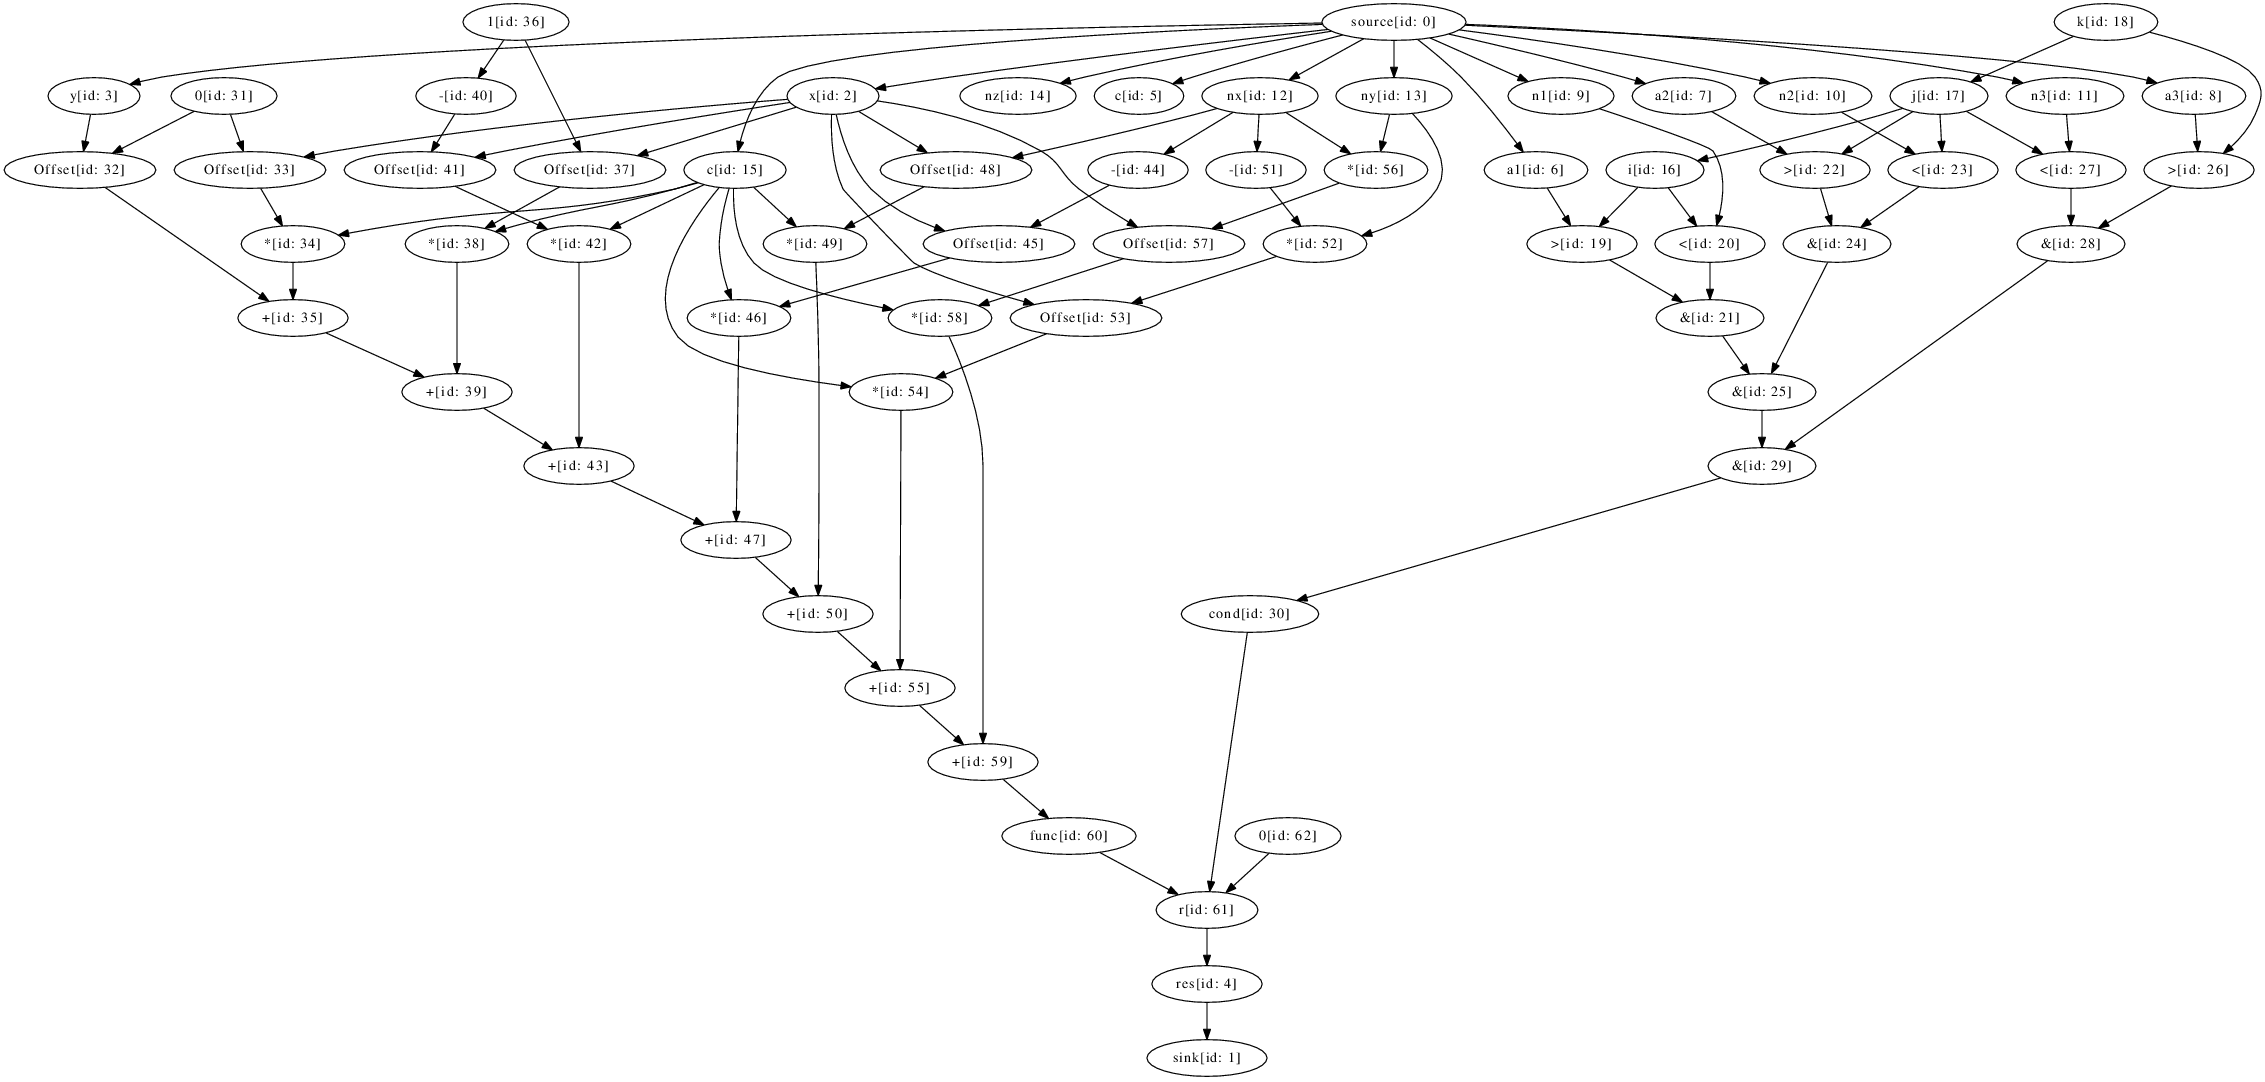
\includegraphics[scale=0.5, clip=true, trim=880 740 650 0]{figs/MaxCtemplateDFG.png}
\caption{Section of a dataflow graph generated using \fastc{}.}
\label{fig:fast-dfg}
\end{figure}


\section{Summary}

We have introduced the \FAST{} language one of the components required
as part of the proposed Aspect-oriented design flow. We have shown the
most important features of the \FAST{} language and how they map to
hardware components on the FPGA based dataflow engine. We have
highlighted the challenges of capturing these constructs with a simple
imperative language such as C and some possible solutions which we
investigate in  \Cref{sec:implementation}.

\Cref{table:feature-comparison1} contrasts the \FAST{} approach
proposed in this project with existing approaches in terms of syntax
and programming paradigm. An imperative, as opposed to functional
paradigm simplifies the language, making it more accessible to novice
users and integrates well with existing application source code. The
dataflow style of the \FAST{} specifications allows for an efficient
specification of designs that map well onto hardware accelerators such
as FPGA-based dataflow engines. The language supports integrated
hardware/software co-design with existing C applications, simplifying
the design exploration process by improving sharing of parameters and
by exposing a unified syntax to external design space exploration
tools (such as the LARA design space exploration flow).

Finally, \Cref{table:feature-comparison2} highlights the support for design
parametrisation and optimisation exploration strategies via the
automated aspect-oriented design flow as opposed to manual
transformations or meta-programming used by existing state-of-the art
compilers.


\begin{table}[!ht]
  \renewcommand{\arraystretch}{1.2}
  \centering
  \begin{tabularx}{\textwidth}{X | p{2.5cm} | p{3cm} | p{1.9cm} }
    \hline
    \bf{Language}                 & \bf{Syntax}              & \bf{Paradigm}               & \bf{Support}              \\
    \hline \hline
    \bf{Lucid}                    & Lucid                    & Functional                  & \multirow{3}{*}{Software} \\
    \cline{1-3}
    \bf{SISAL}                    & SISAL                    & Functional                  &                           \\
    \cline{1-3}
    \bf{Lustre}                   & Lustre                   & Synchronous                 &                           \\
    \bf{MaxCompiler}              & C99(SW) Java(HW)         & Imperative(SW) / Dataflow(HW) & \multirow{3}{*}{Combined} \\
    \bf{Streams-C} \bf{ImpulseC}\ & C99                      & Imperative(SW) / CSP(HW)      &                           \\
    \bf{\FAST{}}/\bf{LARA}        & C99(SW/HW) LARA(Aspects) & Imperative(SW) / Dataflow(HW) &                           \\
  \end{tabularx}
  \caption{Syntax, paradigm and support comparison of the \FAST{}/LARA approach and existing dataflow implementations.}
  \label{table:feature-comparison1}
\end{table}


\begin{table}[!ht]
  \renewcommand{\arraystretch}{1.2}
  \centering
  \begin{tabularx}{\textwidth}{ m{2.5cm} | X | X | p{2.5cm}}
    \hline
    \bf{Language}                  & \bf{Implementation}             & \bf{Design Parametrisation}                     & \bf{Optimisation Strategies}                                                                                                                                        \\
    \hline \hline
    \bf{Lucid}                     & \multirow{3}{*}{Multiprocessor} & \multirow{3}{3cm}{Manual Source Transformation} & \multirow{5}{3cm}{Manual Code Revision}                                                                                                                             \\
   \bf{SISAL}                      &                                 &                                                 &                                                                                                                                                                     \\
 \bf{Lustre}                      &                             &                              &                                                                            \\
    \bf{MaxCompiler}             & \multirow{6}{*}{CPU + FPGA} & Meta-programming             &                                                                            \\
\cline{1-1}\cline{2-3}
  \bf{Streams-C} \bf{ImpulseC}\ &                             & Compiler \newline Directives &                                                                            \\
\hline
  \bf{\FAST{}}/\bf{LARA}         &                             & \multicolumn{2}{p{7cm}}{Compiler Directives + \newline Automated Aspect-Directed Source Transformation} \\
  \end{tabularx}
  \caption{Implementation, parametrisation and optimisations comparison of the \FAST{}/LARA approach and existing dataflow implementations.}
  \label{table:feature-comparison2}
\end{table}
